\documentclass[twoside]{book}

% Packages required by doxygen
\usepackage{calc}
\usepackage{doxygen}
\usepackage{graphicx}
\usepackage[utf8]{inputenc}
\usepackage{makeidx}
\usepackage{multicol}
\usepackage{multirow}
\usepackage{textcomp}
\usepackage[table]{xcolor}

% Font selection
\usepackage[T1]{fontenc}
\usepackage{mathptmx}
\usepackage[scaled=.90]{helvet}
\usepackage{courier}
\usepackage{amssymb}
\usepackage{sectsty}
\renewcommand{\familydefault}{\sfdefault}
\allsectionsfont{%
  \fontseries{bc}\selectfont%
  \color{darkgray}%
}
\renewcommand{\DoxyLabelFont}{%
  \fontseries{bc}\selectfont%
  \color{darkgray}%
}

% Page & text layout
\usepackage{geometry}
\geometry{%
  a4paper,%
  top=2.5cm,%
  bottom=2.5cm,%
  left=2.5cm,%
  right=2.5cm%
}
\tolerance=750
\hfuzz=15pt
\hbadness=750
\setlength{\emergencystretch}{15pt}
\setlength{\parindent}{0cm}
\setlength{\parskip}{0.2cm}
\makeatletter
\renewcommand{\paragraph}{%
  \@startsection{paragraph}{4}{0ex}{-1.0ex}{1.0ex}{%
    \normalfont\normalsize\bfseries\SS@parafont%
  }%
}
\renewcommand{\subparagraph}{%
  \@startsection{subparagraph}{5}{0ex}{-1.0ex}{1.0ex}{%
    \normalfont\normalsize\bfseries\SS@subparafont%
  }%
}
\makeatother

% Headers & footers
\usepackage{fancyhdr}
\pagestyle{fancyplain}
\fancyhead[LE]{\fancyplain{}{\bfseries\thepage}}
\fancyhead[CE]{\fancyplain{}{}}
\fancyhead[RE]{\fancyplain{}{\bfseries\leftmark}}
\fancyhead[LO]{\fancyplain{}{\bfseries\rightmark}}
\fancyhead[CO]{\fancyplain{}{}}
\fancyhead[RO]{\fancyplain{}{\bfseries\thepage}}
\fancyfoot[LE]{\fancyplain{}{}}
\fancyfoot[CE]{\fancyplain{}{}}
\fancyfoot[RE]{\fancyplain{}{\bfseries\scriptsize Generated on Wed Jan 22 2014 12:16:42 for APImeal by Doxygen }}
\fancyfoot[LO]{\fancyplain{}{\bfseries\scriptsize Generated on Wed Jan 22 2014 12:16:42 for APImeal by Doxygen }}
\fancyfoot[CO]{\fancyplain{}{}}
\fancyfoot[RO]{\fancyplain{}{}}
\renewcommand{\footrulewidth}{0.4pt}
\renewcommand{\chaptermark}[1]{%
  \markboth{#1}{}%
}
\renewcommand{\sectionmark}[1]{%
  \markright{\thesection\ #1}%
}

% Indices & bibliography
\usepackage{natbib}
\usepackage[titles]{tocloft}
\setcounter{tocdepth}{3}
\setcounter{secnumdepth}{5}
\makeindex

% Hyperlinks (required, but should be loaded last)
\usepackage{ifpdf}
\ifpdf
  \usepackage[pdftex,pagebackref=true]{hyperref}
\else
  \usepackage[ps2pdf,pagebackref=true]{hyperref}
\fi
\hypersetup{%
  colorlinks=true,%
  linkcolor=blue,%
  citecolor=blue,%
  unicode%
}

% Custom commands
\newcommand{\clearemptydoublepage}{%
  \newpage{\pagestyle{empty}\cleardoublepage}%
}


%===== C O N T E N T S =====

\begin{document}

% Titlepage & ToC
\hypersetup{pageanchor=false}
\pagenumbering{roman}
\begin{titlepage}
\vspace*{7cm}
\begin{center}%
{\Large A\-P\-Imeal \\[1ex]\large 0.\-1 }\\
\vspace*{1cm}
{\large Generated by Doxygen 1.8.4}\\
\vspace*{0.5cm}
{\small Wed Jan 22 2014 12:16:42}\\
\end{center}
\end{titlepage}
\clearemptydoublepage
\tableofcontents
\clearemptydoublepage
\pagenumbering{arabic}
\hypersetup{pageanchor=true}

%--- Begin generated contents ---
\chapter{Hierarchical Index}
\section{Class Hierarchy}
This inheritance list is sorted roughly, but not completely, alphabetically\-:\begin{DoxyCompactList}
\item \contentsline{section}{apimeal\-:\-:A\-Module}{\pageref{classapimeal_1_1AModule}}{}
\item \contentsline{section}{apimeal\-:\-:Error}{\pageref{structapimeal_1_1Error}}{}
\item \contentsline{section}{apimeal\-:\-:I\-Connexion}{\pageref{classapimeal_1_1IConnexion}}{}
\item \contentsline{section}{apimeal\-:\-:I\-Logger}{\pageref{classapimeal_1_1ILogger}}{}
\item \contentsline{section}{apimeal\-:\-:I\-Request}{\pageref{classapimeal_1_1IRequest}}{}
\begin{DoxyCompactList}
\item \contentsline{section}{apimeal\-:\-:I\-Http\-Request}{\pageref{classapimeal_1_1IHttpRequest}}{}
\item \contentsline{section}{apimeal\-:\-:I\-Http\-Response}{\pageref{classapimeal_1_1IHttpResponse}}{}
\end{DoxyCompactList}
\item \contentsline{section}{apimeal\-:\-:Version}{\pageref{structapimeal_1_1Version}}{}
\end{DoxyCompactList}

\chapter{Class Index}
\section{Class List}
Here are the classes, structs, unions and interfaces with brief descriptions\-:\begin{DoxyCompactList}
\item\contentsline{section}{\hyperlink{classapimeal_1_1AModule}{apimeal\-::\-A\-Module} \\*Class which represent the module }{\pageref{classapimeal_1_1AModule}}{}
\item\contentsline{section}{\hyperlink{structapimeal_1_1Error}{apimeal\-::\-Error} \\*Struct for error handling bool Is\-Error (true if there was an error) int Code (error code) std\-::string Message (Message print) }{\pageref{structapimeal_1_1Error}}{}
\item\contentsline{section}{\hyperlink{classapimeal_1_1IConnexion}{apimeal\-::\-I\-Connexion} \\*Class for connecting a client }{\pageref{classapimeal_1_1IConnexion}}{}
\item\contentsline{section}{\hyperlink{classapimeal_1_1IHttpRequest}{apimeal\-::\-I\-Http\-Request} \\*Class for managing request }{\pageref{classapimeal_1_1IHttpRequest}}{}
\item\contentsline{section}{\hyperlink{classapimeal_1_1IHttpResponse}{apimeal\-::\-I\-Http\-Response} \\*Class for create an response request }{\pageref{classapimeal_1_1IHttpResponse}}{}
\item\contentsline{section}{\hyperlink{classapimeal_1_1ILogger}{apimeal\-::\-I\-Logger} \\*Class for logger }{\pageref{classapimeal_1_1ILogger}}{}
\item\contentsline{section}{\hyperlink{classapimeal_1_1IRequest}{apimeal\-::\-I\-Request} \\*Content of a query }{\pageref{classapimeal_1_1IRequest}}{}
\item\contentsline{section}{\hyperlink{structapimeal_1_1Version}{apimeal\-::\-Version} \\*Set the slice versions compatible with the module }{\pageref{structapimeal_1_1Version}}{}
\end{DoxyCompactList}

\chapter{Class Documentation}
\hypertarget{classapimeal_1_1AModule}{\section{apimeal\-:\-:A\-Module Class Reference}
\label{classapimeal_1_1AModule}\index{apimeal\-::\-A\-Module@{apimeal\-::\-A\-Module}}
}


class which represent the module  




{\ttfamily \#include $<$A\-Module.\-hpp$>$}

\subsection*{Public Member Functions}
\begin{DoxyCompactItemize}
\item 
\hyperlink{classapimeal_1_1AModule_af499c09d8c815150cd4ab48947e7325c}{A\-Module} (\hyperlink{classapimeal_1_1ILogger}{I\-Logger} $\ast$log)
\begin{DoxyCompactList}\small\item\em Constructor Constructor of class \hyperlink{classapimeal_1_1AModule}{A\-Module}. \end{DoxyCompactList}\item 
\hypertarget{classapimeal_1_1AModule_adab8d8b39d08162ba4c9bf9e609f243b}{virtual \hyperlink{classapimeal_1_1AModule_adab8d8b39d08162ba4c9bf9e609f243b}{$\sim$\-A\-Module} ()}\label{classapimeal_1_1AModule_adab8d8b39d08162ba4c9bf9e609f243b}

\begin{DoxyCompactList}\small\item\em Destructor Destructor of class \hyperlink{classapimeal_1_1AModule}{A\-Module}. \end{DoxyCompactList}\item 
virtual std\-::map$<$ e\-Type\-Module, \\*
e\-Priority $>$ \hyperlink{classapimeal_1_1AModule_a86c37e1e56fa8b44d86e446630a731cb}{get\-Priority} () const =0
\begin{DoxyCompactList}\small\item\em Get map of module's priority. \end{DoxyCompactList}\item 
virtual \hyperlink{structapimeal_1_1Version}{Version} const \& \hyperlink{classapimeal_1_1AModule_a7567906eea190833d73f77f1da848b69}{get\-Version} () const =0
\begin{DoxyCompactList}\small\item\em Get version of the module. \end{DoxyCompactList}\item 
virtual std\-::string const \& \hyperlink{classapimeal_1_1AModule_ace61580f63d9c256df7659f23c471afc}{get\-Name} () const =0
\begin{DoxyCompactList}\small\item\em Get name of module. \end{DoxyCompactList}\item 
virtual void \hyperlink{classapimeal_1_1AModule_a5a6614e5e72edb9c5df2b92e1ece869a}{pre\-Connexion} (\hyperlink{classapimeal_1_1IConnexion}{I\-Connexion} $\ast$, \hyperlink{structapimeal_1_1Error}{Error} \&)
\begin{DoxyCompactList}\small\item\em Before connexion. \end{DoxyCompactList}\item 
virtual void \hyperlink{classapimeal_1_1AModule_aca21d0bfefef5455fcd6dd6f907fe283}{post\-Connexion} (\hyperlink{classapimeal_1_1IConnexion}{I\-Connexion} $\ast$, \hyperlink{structapimeal_1_1Error}{Error} \&)
\begin{DoxyCompactList}\small\item\em After connexion. \end{DoxyCompactList}\item 
virtual void \hyperlink{classapimeal_1_1AModule_afdc72a0d20e2e8d7c6bc738413981acc}{pre\-Parse\-Request} (\hyperlink{classapimeal_1_1IHttpRequest}{I\-Http\-Request} $\ast$, \hyperlink{structapimeal_1_1Error}{Error} \&)
\begin{DoxyCompactList}\small\item\em Before parsing a query. \end{DoxyCompactList}\item 
virtual void \hyperlink{classapimeal_1_1AModule_a2826a882eda9e5e7b5b6ca6b1051a479}{post\-Parse\-Request} (\hyperlink{classapimeal_1_1IHttpRequest}{I\-Http\-Request} $\ast$, \hyperlink{structapimeal_1_1Error}{Error} \&)
\begin{DoxyCompactList}\small\item\em After parsing a request. \end{DoxyCompactList}\item 
virtual void \hyperlink{classapimeal_1_1AModule_a01660e7d5ed59a20e9a81e03958a9911}{content\-Module} (\hyperlink{classapimeal_1_1IHttpRequest}{I\-Http\-Request} $\ast$, \hyperlink{structapimeal_1_1Error}{Error} \&)
\begin{DoxyCompactList}\small\item\em Get body of the request. \end{DoxyCompactList}\item 
virtual void \hyperlink{classapimeal_1_1AModule_aab6161ce426b4ee31b8e17bdcdfcbfea}{C\-G\-I\-Module} (\hyperlink{classapimeal_1_1IHttpResponse}{I\-Http\-Response} $\ast$, \hyperlink{structapimeal_1_1Error}{Error} \&)
\begin{DoxyCompactList}\small\item\em Manage of Common Gateway Interface. \end{DoxyCompactList}\item 
virtual void \hyperlink{classapimeal_1_1AModule_ab245f944a40f67dddb5777864677468d}{post\-Generate\-Response} (\hyperlink{classapimeal_1_1IHttpResponse}{I\-Http\-Response} $\ast$, \hyperlink{structapimeal_1_1Error}{Error} \&)
\begin{DoxyCompactList}\small\item\em After generation of the response. \end{DoxyCompactList}\item 
virtual void \hyperlink{classapimeal_1_1AModule_a22ad5b93999ee07024a42aadcd9604e0}{pre\-Send\-Request} (\hyperlink{classapimeal_1_1IHttpResponse}{I\-Http\-Response} $\ast$, \hyperlink{classapimeal_1_1IConnexion}{I\-Connexion} $\ast$, \hyperlink{structapimeal_1_1Error}{Error} \&)
\begin{DoxyCompactList}\small\item\em Before sending the response. \end{DoxyCompactList}\item 
\hypertarget{classapimeal_1_1AModule_adc7136919b05fbde2f0f3b4d3d1bc844}{virtual void \hyperlink{classapimeal_1_1AModule_adc7136919b05fbde2f0f3b4d3d1bc844}{release} ()}\label{classapimeal_1_1AModule_adc7136919b05fbde2f0f3b4d3d1bc844}

\begin{DoxyCompactList}\small\item\em Free memory. \end{DoxyCompactList}\end{DoxyCompactItemize}
\subsection*{Protected Attributes}
\begin{DoxyCompactItemize}
\item 
\hyperlink{classapimeal_1_1ILogger}{I\-Logger} $\ast$ \hyperlink{classapimeal_1_1AModule_a2c29f9418997cf7e82715bc09c8dcca2}{\-\_\-logger}
\end{DoxyCompactItemize}


\subsection{Detailed Description}
class which represent the module 

\subsection{Constructor \& Destructor Documentation}
\hypertarget{classapimeal_1_1AModule_af499c09d8c815150cd4ab48947e7325c}{\index{apimeal\-::\-A\-Module@{apimeal\-::\-A\-Module}!A\-Module@{A\-Module}}
\index{A\-Module@{A\-Module}!apimeal::AModule@{apimeal\-::\-A\-Module}}
\subsubsection[{A\-Module}]{\setlength{\rightskip}{0pt plus 5cm}apimeal\-::\-A\-Module\-::\-A\-Module (
\begin{DoxyParamCaption}
\item[{{\bf I\-Logger} $\ast$}]{log}
\end{DoxyParamCaption}
)\hspace{0.3cm}{\ttfamily [inline]}}}\label{classapimeal_1_1AModule_af499c09d8c815150cd4ab48947e7325c}


Constructor Constructor of class \hyperlink{classapimeal_1_1AModule}{A\-Module}. 


\begin{DoxyParams}{Parameters}
{\em log} & \-: Logger link with the module \\
\hline
\end{DoxyParams}


\subsection{Member Function Documentation}
\hypertarget{classapimeal_1_1AModule_aab6161ce426b4ee31b8e17bdcdfcbfea}{\index{apimeal\-::\-A\-Module@{apimeal\-::\-A\-Module}!C\-G\-I\-Module@{C\-G\-I\-Module}}
\index{C\-G\-I\-Module@{C\-G\-I\-Module}!apimeal::AModule@{apimeal\-::\-A\-Module}}
\subsubsection[{C\-G\-I\-Module}]{\setlength{\rightskip}{0pt plus 5cm}virtual void apimeal\-::\-A\-Module\-::\-C\-G\-I\-Module (
\begin{DoxyParamCaption}
\item[{{\bf I\-Http\-Response} $\ast$}]{, }
\item[{{\bf Error} \&}]{}
\end{DoxyParamCaption}
)\hspace{0.3cm}{\ttfamily [inline]}, {\ttfamily [virtual]}}}\label{classapimeal_1_1AModule_aab6161ce426b4ee31b8e17bdcdfcbfea}


Manage of Common Gateway Interface. 


\begin{DoxyParams}{Parameters}
{\em \hyperlink{classapimeal_1_1IHttpResponse}{I\-Http\-Response}} & \-: Class for manage a query \\
\hline
{\em \hyperlink{structapimeal_1_1Error}{Error}} & \-: Class for manage an error \\
\hline
\end{DoxyParams}
\hypertarget{classapimeal_1_1AModule_a01660e7d5ed59a20e9a81e03958a9911}{\index{apimeal\-::\-A\-Module@{apimeal\-::\-A\-Module}!content\-Module@{content\-Module}}
\index{content\-Module@{content\-Module}!apimeal::AModule@{apimeal\-::\-A\-Module}}
\subsubsection[{content\-Module}]{\setlength{\rightskip}{0pt plus 5cm}virtual void apimeal\-::\-A\-Module\-::content\-Module (
\begin{DoxyParamCaption}
\item[{{\bf I\-Http\-Request} $\ast$}]{, }
\item[{{\bf Error} \&}]{}
\end{DoxyParamCaption}
)\hspace{0.3cm}{\ttfamily [inline]}, {\ttfamily [virtual]}}}\label{classapimeal_1_1AModule_a01660e7d5ed59a20e9a81e03958a9911}


Get body of the request. 


\begin{DoxyParams}{Parameters}
{\em \hyperlink{classapimeal_1_1IHttpRequest}{I\-Http\-Request}} & \-: Class for manage a query \\
\hline
{\em \hyperlink{structapimeal_1_1Error}{Error}} & \-: Class for manage an error \\
\hline
\end{DoxyParams}
\hypertarget{classapimeal_1_1AModule_ace61580f63d9c256df7659f23c471afc}{\index{apimeal\-::\-A\-Module@{apimeal\-::\-A\-Module}!get\-Name@{get\-Name}}
\index{get\-Name@{get\-Name}!apimeal::AModule@{apimeal\-::\-A\-Module}}
\subsubsection[{get\-Name}]{\setlength{\rightskip}{0pt plus 5cm}virtual std\-::string const\& apimeal\-::\-A\-Module\-::get\-Name (
\begin{DoxyParamCaption}
{}
\end{DoxyParamCaption}
) const\hspace{0.3cm}{\ttfamily [pure virtual]}}}\label{classapimeal_1_1AModule_ace61580f63d9c256df7659f23c471afc}


Get name of module. 

\begin{DoxyReturn}{Returns}
String with the module's name 
\end{DoxyReturn}
\hypertarget{classapimeal_1_1AModule_a86c37e1e56fa8b44d86e446630a731cb}{\index{apimeal\-::\-A\-Module@{apimeal\-::\-A\-Module}!get\-Priority@{get\-Priority}}
\index{get\-Priority@{get\-Priority}!apimeal::AModule@{apimeal\-::\-A\-Module}}
\subsubsection[{get\-Priority}]{\setlength{\rightskip}{0pt plus 5cm}virtual std\-::map$<$e\-Type\-Module, e\-Priority$>$ apimeal\-::\-A\-Module\-::get\-Priority (
\begin{DoxyParamCaption}
{}
\end{DoxyParamCaption}
) const\hspace{0.3cm}{\ttfamily [pure virtual]}}}\label{classapimeal_1_1AModule_a86c37e1e56fa8b44d86e446630a731cb}


Get map of module's priority. 

\begin{DoxyReturn}{Returns}
Map of priority of module 
\end{DoxyReturn}
\hypertarget{classapimeal_1_1AModule_a7567906eea190833d73f77f1da848b69}{\index{apimeal\-::\-A\-Module@{apimeal\-::\-A\-Module}!get\-Version@{get\-Version}}
\index{get\-Version@{get\-Version}!apimeal::AModule@{apimeal\-::\-A\-Module}}
\subsubsection[{get\-Version}]{\setlength{\rightskip}{0pt plus 5cm}virtual {\bf Version} const\& apimeal\-::\-A\-Module\-::get\-Version (
\begin{DoxyParamCaption}
{}
\end{DoxyParamCaption}
) const\hspace{0.3cm}{\ttfamily [pure virtual]}}}\label{classapimeal_1_1AModule_a7567906eea190833d73f77f1da848b69}


Get version of the module. 

\begin{DoxyReturn}{Returns}
\hyperlink{structapimeal_1_1Version}{Version} of the module 
\end{DoxyReturn}
\hypertarget{classapimeal_1_1AModule_aca21d0bfefef5455fcd6dd6f907fe283}{\index{apimeal\-::\-A\-Module@{apimeal\-::\-A\-Module}!post\-Connexion@{post\-Connexion}}
\index{post\-Connexion@{post\-Connexion}!apimeal::AModule@{apimeal\-::\-A\-Module}}
\subsubsection[{post\-Connexion}]{\setlength{\rightskip}{0pt plus 5cm}virtual void apimeal\-::\-A\-Module\-::post\-Connexion (
\begin{DoxyParamCaption}
\item[{{\bf I\-Connexion} $\ast$}]{, }
\item[{{\bf Error} \&}]{}
\end{DoxyParamCaption}
)\hspace{0.3cm}{\ttfamily [inline]}, {\ttfamily [virtual]}}}\label{classapimeal_1_1AModule_aca21d0bfefef5455fcd6dd6f907fe283}


After connexion. 


\begin{DoxyParams}{Parameters}
{\em \hyperlink{classapimeal_1_1IConnexion}{I\-Connexion}} & \-: Class for connecting a client \\
\hline
{\em \hyperlink{structapimeal_1_1Error}{Error}} & \-: Class for manage an error \\
\hline
\end{DoxyParams}
\hypertarget{classapimeal_1_1AModule_ab245f944a40f67dddb5777864677468d}{\index{apimeal\-::\-A\-Module@{apimeal\-::\-A\-Module}!post\-Generate\-Response@{post\-Generate\-Response}}
\index{post\-Generate\-Response@{post\-Generate\-Response}!apimeal::AModule@{apimeal\-::\-A\-Module}}
\subsubsection[{post\-Generate\-Response}]{\setlength{\rightskip}{0pt plus 5cm}virtual void apimeal\-::\-A\-Module\-::post\-Generate\-Response (
\begin{DoxyParamCaption}
\item[{{\bf I\-Http\-Response} $\ast$}]{, }
\item[{{\bf Error} \&}]{}
\end{DoxyParamCaption}
)\hspace{0.3cm}{\ttfamily [inline]}, {\ttfamily [virtual]}}}\label{classapimeal_1_1AModule_ab245f944a40f67dddb5777864677468d}


After generation of the response. 


\begin{DoxyParams}{Parameters}
{\em \hyperlink{classapimeal_1_1IHttpResponse}{I\-Http\-Response}} & \-: Class with the query response \\
\hline
{\em \hyperlink{structapimeal_1_1Error}{Error}} & \-: Class for manage an error \\
\hline
\end{DoxyParams}
\hypertarget{classapimeal_1_1AModule_a2826a882eda9e5e7b5b6ca6b1051a479}{\index{apimeal\-::\-A\-Module@{apimeal\-::\-A\-Module}!post\-Parse\-Request@{post\-Parse\-Request}}
\index{post\-Parse\-Request@{post\-Parse\-Request}!apimeal::AModule@{apimeal\-::\-A\-Module}}
\subsubsection[{post\-Parse\-Request}]{\setlength{\rightskip}{0pt plus 5cm}virtual void apimeal\-::\-A\-Module\-::post\-Parse\-Request (
\begin{DoxyParamCaption}
\item[{{\bf I\-Http\-Request} $\ast$}]{, }
\item[{{\bf Error} \&}]{}
\end{DoxyParamCaption}
)\hspace{0.3cm}{\ttfamily [inline]}, {\ttfamily [virtual]}}}\label{classapimeal_1_1AModule_a2826a882eda9e5e7b5b6ca6b1051a479}


After parsing a request. 


\begin{DoxyParams}{Parameters}
{\em \hyperlink{classapimeal_1_1IHttpRequest}{I\-Http\-Request}} & \-: Class for manage a query \\
\hline
{\em \hyperlink{structapimeal_1_1Error}{Error}} & \-: Class for manage an error \\
\hline
\end{DoxyParams}
\hypertarget{classapimeal_1_1AModule_a5a6614e5e72edb9c5df2b92e1ece869a}{\index{apimeal\-::\-A\-Module@{apimeal\-::\-A\-Module}!pre\-Connexion@{pre\-Connexion}}
\index{pre\-Connexion@{pre\-Connexion}!apimeal::AModule@{apimeal\-::\-A\-Module}}
\subsubsection[{pre\-Connexion}]{\setlength{\rightskip}{0pt plus 5cm}virtual void apimeal\-::\-A\-Module\-::pre\-Connexion (
\begin{DoxyParamCaption}
\item[{{\bf I\-Connexion} $\ast$}]{, }
\item[{{\bf Error} \&}]{}
\end{DoxyParamCaption}
)\hspace{0.3cm}{\ttfamily [inline]}, {\ttfamily [virtual]}}}\label{classapimeal_1_1AModule_a5a6614e5e72edb9c5df2b92e1ece869a}


Before connexion. 


\begin{DoxyParams}{Parameters}
{\em \hyperlink{classapimeal_1_1IConnexion}{I\-Connexion}} & \-: Class for connecting a client \\
\hline
{\em \hyperlink{structapimeal_1_1Error}{Error}} & \-: Class for manage an error \\
\hline
\end{DoxyParams}
\hypertarget{classapimeal_1_1AModule_afdc72a0d20e2e8d7c6bc738413981acc}{\index{apimeal\-::\-A\-Module@{apimeal\-::\-A\-Module}!pre\-Parse\-Request@{pre\-Parse\-Request}}
\index{pre\-Parse\-Request@{pre\-Parse\-Request}!apimeal::AModule@{apimeal\-::\-A\-Module}}
\subsubsection[{pre\-Parse\-Request}]{\setlength{\rightskip}{0pt plus 5cm}virtual void apimeal\-::\-A\-Module\-::pre\-Parse\-Request (
\begin{DoxyParamCaption}
\item[{{\bf I\-Http\-Request} $\ast$}]{, }
\item[{{\bf Error} \&}]{}
\end{DoxyParamCaption}
)\hspace{0.3cm}{\ttfamily [inline]}, {\ttfamily [virtual]}}}\label{classapimeal_1_1AModule_afdc72a0d20e2e8d7c6bc738413981acc}


Before parsing a query. 


\begin{DoxyParams}{Parameters}
{\em \hyperlink{classapimeal_1_1IHttpRequest}{I\-Http\-Request}} & \-: Class for manage a query \\
\hline
{\em \hyperlink{structapimeal_1_1Error}{Error}} & \-: Class for manage an error \\
\hline
\end{DoxyParams}
\hypertarget{classapimeal_1_1AModule_a22ad5b93999ee07024a42aadcd9604e0}{\index{apimeal\-::\-A\-Module@{apimeal\-::\-A\-Module}!pre\-Send\-Request@{pre\-Send\-Request}}
\index{pre\-Send\-Request@{pre\-Send\-Request}!apimeal::AModule@{apimeal\-::\-A\-Module}}
\subsubsection[{pre\-Send\-Request}]{\setlength{\rightskip}{0pt plus 5cm}virtual void apimeal\-::\-A\-Module\-::pre\-Send\-Request (
\begin{DoxyParamCaption}
\item[{{\bf I\-Http\-Response} $\ast$}]{, }
\item[{{\bf I\-Connexion} $\ast$}]{, }
\item[{{\bf Error} \&}]{}
\end{DoxyParamCaption}
)\hspace{0.3cm}{\ttfamily [inline]}, {\ttfamily [virtual]}}}\label{classapimeal_1_1AModule_a22ad5b93999ee07024a42aadcd9604e0}


Before sending the response. 


\begin{DoxyParams}{Parameters}
{\em \hyperlink{classapimeal_1_1IHttpResponse}{I\-Http\-Response}} & \-: Class with the query response \\
\hline
{\em \hyperlink{classapimeal_1_1IConnexion}{I\-Connexion}} & \-: Class with the query response \\
\hline
{\em \hyperlink{structapimeal_1_1Error}{Error}} & \-: Class for manage an error \\
\hline
\end{DoxyParams}


\subsection{Member Data Documentation}
\hypertarget{classapimeal_1_1AModule_a2c29f9418997cf7e82715bc09c8dcca2}{\index{apimeal\-::\-A\-Module@{apimeal\-::\-A\-Module}!\-\_\-logger@{\-\_\-logger}}
\index{\-\_\-logger@{\-\_\-logger}!apimeal::AModule@{apimeal\-::\-A\-Module}}
\subsubsection[{\-\_\-logger}]{\setlength{\rightskip}{0pt plus 5cm}{\bf I\-Logger}$\ast$ apimeal\-::\-A\-Module\-::\-\_\-logger\hspace{0.3cm}{\ttfamily [protected]}}}\label{classapimeal_1_1AModule_a2c29f9418997cf7e82715bc09c8dcca2}
Logger 

The documentation for this class was generated from the following file\-:\begin{DoxyCompactItemize}
\item 
/home/corpille/\-Documents/\-Zia/apimeal/include/apimeal/A\-Module.\-hpp\end{DoxyCompactItemize}

\hypertarget{structapimeal_1_1Error}{\section{apimeal\-:\-:Error Struct Reference}
\label{structapimeal_1_1Error}\index{apimeal\-::\-Error@{apimeal\-::\-Error}}
}


Struct for error handling bool Is\-Error (true if there was an error) int Code (error code) std\-::string Message (Message print)  




{\ttfamily \#include $<$Error.\-hpp$>$}

\subsection*{Public Attributes}
\begin{DoxyCompactItemize}
\item 
\hypertarget{structapimeal_1_1Error_a478d14ea80925fae993aa652b8dc6fb4}{bool {\bfseries Is\-Error}}\label{structapimeal_1_1Error_a478d14ea80925fae993aa652b8dc6fb4}

\item 
\hypertarget{structapimeal_1_1Error_a4dd936b868553fca14e910c33bb81bc2}{int {\bfseries Code}}\label{structapimeal_1_1Error_a4dd936b868553fca14e910c33bb81bc2}

\item 
\hypertarget{structapimeal_1_1Error_a28eff246cdeb42c782cb207e4e535472}{std\-::string {\bfseries Message}}\label{structapimeal_1_1Error_a28eff246cdeb42c782cb207e4e535472}

\end{DoxyCompactItemize}


\subsection{Detailed Description}
Struct for error handling bool Is\-Error (true if there was an error) int Code (error code) std\-::string Message (Message print) 

The documentation for this struct was generated from the following file\-:\begin{DoxyCompactItemize}
\item 
/home/corpille/\-Documents/\-Zia/apimeal/include/apimeal/Error.\-hpp\end{DoxyCompactItemize}

\hypertarget{classapimeal_1_1IConnexion}{\section{apimeal\-:\-:I\-Connexion Class Reference}
\label{classapimeal_1_1IConnexion}\index{apimeal\-::\-I\-Connexion@{apimeal\-::\-I\-Connexion}}
}


Class for connecting a client.  




{\ttfamily \#include $<$I\-Connexion.\-hpp$>$}

\subsection*{Public Member Functions}
\begin{DoxyCompactItemize}
\item 
\hypertarget{classapimeal_1_1IConnexion_afa1d85aeadc451143eef2837d5ea4939}{virtual \hyperlink{classapimeal_1_1IConnexion_afa1d85aeadc451143eef2837d5ea4939}{$\sim$\-I\-Connexion} ()}\label{classapimeal_1_1IConnexion_afa1d85aeadc451143eef2837d5ea4939}

\begin{DoxyCompactList}\small\item\em Destructor virtuel. \end{DoxyCompactList}\item 
virtual std\-::string const \& \hyperlink{classapimeal_1_1IConnexion_a8ab3c43f9e1356ed9d46a30ff86ee093}{get\-Hostname} () const =0
\begin{DoxyCompactList}\small\item\em get\-Hostname \end{DoxyCompactList}\item 
virtual std\-::string const \& \hyperlink{classapimeal_1_1IConnexion_a6504bb6018c8ddb8cf367384a0b7b178}{get\-Ip} () const =0
\begin{DoxyCompactList}\small\item\em get\-Ip \end{DoxyCompactList}\item 
virtual int \hyperlink{classapimeal_1_1IConnexion_a405c77b84198d491f20e79a0fcb4d133}{get\-Port} () const =0
\begin{DoxyCompactList}\small\item\em get\-Port \end{DoxyCompactList}\item 
virtual std\-::string const \& \hyperlink{classapimeal_1_1IConnexion_ae1a0352ab450dea6afd278385747f750}{get\-Request} () const =0
\begin{DoxyCompactList}\small\item\em get the Request \end{DoxyCompactList}\item 
virtual void \hyperlink{classapimeal_1_1IConnexion_aba7b8303d379e629b59f49621fd6b704}{set\-Request} (std\-::string const \&request)=0
\begin{DoxyCompactList}\small\item\em set the Request \end{DoxyCompactList}\end{DoxyCompactItemize}


\subsection{Detailed Description}
Class for connecting a client. 

\subsection{Member Function Documentation}
\hypertarget{classapimeal_1_1IConnexion_a8ab3c43f9e1356ed9d46a30ff86ee093}{\index{apimeal\-::\-I\-Connexion@{apimeal\-::\-I\-Connexion}!get\-Hostname@{get\-Hostname}}
\index{get\-Hostname@{get\-Hostname}!apimeal::IConnexion@{apimeal\-::\-I\-Connexion}}
\subsubsection[{get\-Hostname}]{\setlength{\rightskip}{0pt plus 5cm}virtual std\-::string const\& apimeal\-::\-I\-Connexion\-::get\-Hostname (
\begin{DoxyParamCaption}
{}
\end{DoxyParamCaption}
) const\hspace{0.3cm}{\ttfamily [pure virtual]}}}\label{classapimeal_1_1IConnexion_a8ab3c43f9e1356ed9d46a30ff86ee093}


get\-Hostname 

\begin{DoxyReturn}{Returns}
std\-::string const \& \-: Hostname client 
\end{DoxyReturn}
\hypertarget{classapimeal_1_1IConnexion_a6504bb6018c8ddb8cf367384a0b7b178}{\index{apimeal\-::\-I\-Connexion@{apimeal\-::\-I\-Connexion}!get\-Ip@{get\-Ip}}
\index{get\-Ip@{get\-Ip}!apimeal::IConnexion@{apimeal\-::\-I\-Connexion}}
\subsubsection[{get\-Ip}]{\setlength{\rightskip}{0pt plus 5cm}virtual std\-::string const\& apimeal\-::\-I\-Connexion\-::get\-Ip (
\begin{DoxyParamCaption}
{}
\end{DoxyParamCaption}
) const\hspace{0.3cm}{\ttfamily [pure virtual]}}}\label{classapimeal_1_1IConnexion_a6504bb6018c8ddb8cf367384a0b7b178}


get\-Ip 

\begin{DoxyReturn}{Returns}
std\-::string const \& \-: Ip client ex (192.\-168.\-0.\-1) 
\end{DoxyReturn}
\hypertarget{classapimeal_1_1IConnexion_a405c77b84198d491f20e79a0fcb4d133}{\index{apimeal\-::\-I\-Connexion@{apimeal\-::\-I\-Connexion}!get\-Port@{get\-Port}}
\index{get\-Port@{get\-Port}!apimeal::IConnexion@{apimeal\-::\-I\-Connexion}}
\subsubsection[{get\-Port}]{\setlength{\rightskip}{0pt plus 5cm}virtual int apimeal\-::\-I\-Connexion\-::get\-Port (
\begin{DoxyParamCaption}
{}
\end{DoxyParamCaption}
) const\hspace{0.3cm}{\ttfamily [pure virtual]}}}\label{classapimeal_1_1IConnexion_a405c77b84198d491f20e79a0fcb4d133}


get\-Port 

\begin{DoxyReturn}{Returns}
int \-: Port client 
\end{DoxyReturn}
\hypertarget{classapimeal_1_1IConnexion_ae1a0352ab450dea6afd278385747f750}{\index{apimeal\-::\-I\-Connexion@{apimeal\-::\-I\-Connexion}!get\-Request@{get\-Request}}
\index{get\-Request@{get\-Request}!apimeal::IConnexion@{apimeal\-::\-I\-Connexion}}
\subsubsection[{get\-Request}]{\setlength{\rightskip}{0pt plus 5cm}virtual std\-::string const\& apimeal\-::\-I\-Connexion\-::get\-Request (
\begin{DoxyParamCaption}
{}
\end{DoxyParamCaption}
) const\hspace{0.3cm}{\ttfamily [pure virtual]}}}\label{classapimeal_1_1IConnexion_ae1a0352ab450dea6afd278385747f750}


get the Request 

\begin{DoxyReturn}{Returns}
std\-::string const \& \-: Request client 
\end{DoxyReturn}
\hypertarget{classapimeal_1_1IConnexion_aba7b8303d379e629b59f49621fd6b704}{\index{apimeal\-::\-I\-Connexion@{apimeal\-::\-I\-Connexion}!set\-Request@{set\-Request}}
\index{set\-Request@{set\-Request}!apimeal::IConnexion@{apimeal\-::\-I\-Connexion}}
\subsubsection[{set\-Request}]{\setlength{\rightskip}{0pt plus 5cm}virtual void apimeal\-::\-I\-Connexion\-::set\-Request (
\begin{DoxyParamCaption}
\item[{std\-::string const \&}]{request}
\end{DoxyParamCaption}
)\hspace{0.3cm}{\ttfamily [pure virtual]}}}\label{classapimeal_1_1IConnexion_aba7b8303d379e629b59f49621fd6b704}


set the Request 


\begin{DoxyParams}{Parameters}
{\em std\-::string} & const \& request \-: The request \\
\hline
\end{DoxyParams}
\begin{DoxyReturn}{Returns}
void 
\end{DoxyReturn}


The documentation for this class was generated from the following file\-:\begin{DoxyCompactItemize}
\item 
/home/corpille/\-Documents/\-Zia/apimeal/include/apimeal/I\-Connexion.\-hpp\end{DoxyCompactItemize}

\hypertarget{classapimeal_1_1IHttpRequest}{\section{apimeal\-:\-:I\-Http\-Request Class Reference}
\label{classapimeal_1_1IHttpRequest}\index{apimeal\-::\-I\-Http\-Request@{apimeal\-::\-I\-Http\-Request}}
}


class for managing request  




{\ttfamily \#include $<$I\-Http\-Request.\-hpp$>$}

Inheritance diagram for apimeal\-:\-:I\-Http\-Request\-:\begin{figure}[H]
\begin{center}
\leavevmode
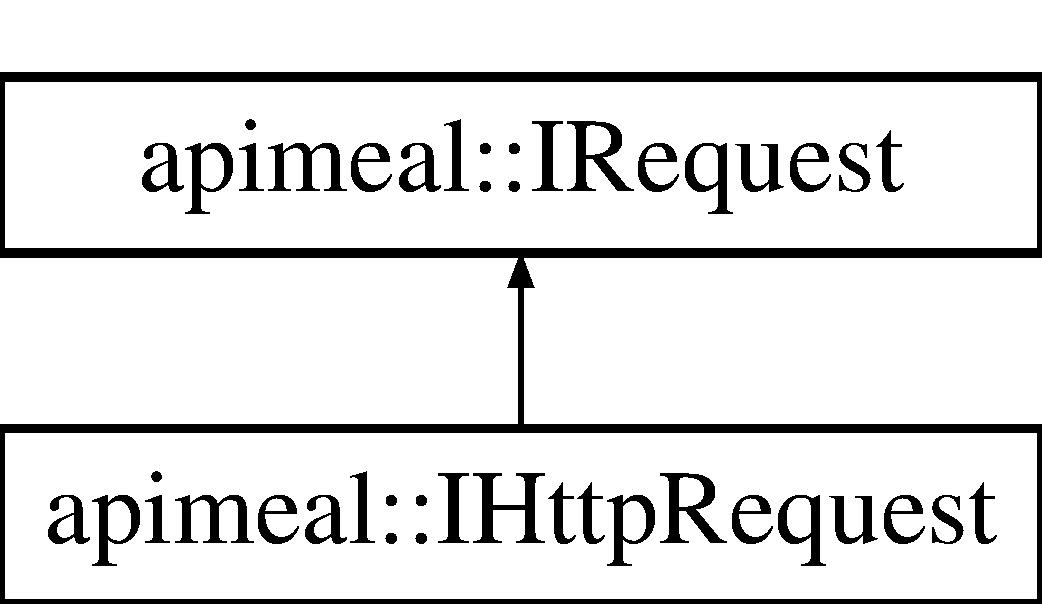
\includegraphics[height=2.000000cm]{classapimeal_1_1IHttpRequest}
\end{center}
\end{figure}
\subsection*{Public Member Functions}
\begin{DoxyCompactItemize}
\item 
\hypertarget{classapimeal_1_1IHttpRequest_a75d1d8b94d7a06e2cd06f9f381e1ffe8}{virtual \hyperlink{classapimeal_1_1IHttpRequest_a75d1d8b94d7a06e2cd06f9f381e1ffe8}{$\sim$\-I\-Http\-Request} ()}\label{classapimeal_1_1IHttpRequest_a75d1d8b94d7a06e2cd06f9f381e1ffe8}

\begin{DoxyCompactList}\small\item\em Destructor. \end{DoxyCompactList}\item 
virtual void \hyperlink{classapimeal_1_1IHttpRequest_a19de02fe350e31b7b21b2b9e16054f26}{set\-Method} (std\-::string const \&)=0
\begin{DoxyCompactList}\small\item\em Setter for \-\_\-method. \end{DoxyCompactList}\item 
virtual std\-::string const \& \hyperlink{classapimeal_1_1IHttpRequest_a397ada95584df34288f026a368c94630}{get\-Method} () const =0
\begin{DoxyCompactList}\small\item\em Getter for \-\_\-method. \end{DoxyCompactList}\item 
virtual void \hyperlink{classapimeal_1_1IHttpRequest_a00c82fbfd32e54cf4ea0db7ea3200662}{set\-Request\-U\-R\-I} (std\-::string const \&)=0
\begin{DoxyCompactList}\small\item\em Setter for \-\_\-request\-U\-R\-I. \end{DoxyCompactList}\item 
virtual std\-::string const \& \hyperlink{classapimeal_1_1IHttpRequest_adade2c139e4701f2777dd8304c88aa4c}{get\-Request\-U\-R\-I} () const =0
\begin{DoxyCompactList}\small\item\em Getter for \-\_\-request\-U\-R\-I. \end{DoxyCompactList}\end{DoxyCompactItemize}


\subsection{Detailed Description}
class for managing request 

\subsection{Member Function Documentation}
\hypertarget{classapimeal_1_1IHttpRequest_a397ada95584df34288f026a368c94630}{\index{apimeal\-::\-I\-Http\-Request@{apimeal\-::\-I\-Http\-Request}!get\-Method@{get\-Method}}
\index{get\-Method@{get\-Method}!apimeal::IHttpRequest@{apimeal\-::\-I\-Http\-Request}}
\subsubsection[{get\-Method}]{\setlength{\rightskip}{0pt plus 5cm}virtual std\-::string const\& apimeal\-::\-I\-Http\-Request\-::get\-Method (
\begin{DoxyParamCaption}
{}
\end{DoxyParamCaption}
) const\hspace{0.3cm}{\ttfamily [pure virtual]}}}\label{classapimeal_1_1IHttpRequest_a397ada95584df34288f026a368c94630}


Getter for \-\_\-method. 

\begin{DoxyReturn}{Returns}
std\-::string const \& \-: method 
\end{DoxyReturn}
\hypertarget{classapimeal_1_1IHttpRequest_adade2c139e4701f2777dd8304c88aa4c}{\index{apimeal\-::\-I\-Http\-Request@{apimeal\-::\-I\-Http\-Request}!get\-Request\-U\-R\-I@{get\-Request\-U\-R\-I}}
\index{get\-Request\-U\-R\-I@{get\-Request\-U\-R\-I}!apimeal::IHttpRequest@{apimeal\-::\-I\-Http\-Request}}
\subsubsection[{get\-Request\-U\-R\-I}]{\setlength{\rightskip}{0pt plus 5cm}virtual std\-::string const\& apimeal\-::\-I\-Http\-Request\-::get\-Request\-U\-R\-I (
\begin{DoxyParamCaption}
{}
\end{DoxyParamCaption}
) const\hspace{0.3cm}{\ttfamily [pure virtual]}}}\label{classapimeal_1_1IHttpRequest_adade2c139e4701f2777dd8304c88aa4c}


Getter for \-\_\-request\-U\-R\-I. 

\begin{DoxyReturn}{Returns}
std\-::string const \& \-: request\-U\-R\-I 
\end{DoxyReturn}
\hypertarget{classapimeal_1_1IHttpRequest_a19de02fe350e31b7b21b2b9e16054f26}{\index{apimeal\-::\-I\-Http\-Request@{apimeal\-::\-I\-Http\-Request}!set\-Method@{set\-Method}}
\index{set\-Method@{set\-Method}!apimeal::IHttpRequest@{apimeal\-::\-I\-Http\-Request}}
\subsubsection[{set\-Method}]{\setlength{\rightskip}{0pt plus 5cm}virtual void apimeal\-::\-I\-Http\-Request\-::set\-Method (
\begin{DoxyParamCaption}
\item[{std\-::string const \&}]{}
\end{DoxyParamCaption}
)\hspace{0.3cm}{\ttfamily [pure virtual]}}}\label{classapimeal_1_1IHttpRequest_a19de02fe350e31b7b21b2b9e16054f26}


Setter for \-\_\-method. 


\begin{DoxyParams}{Parameters}
{\em std\-::string} & const \& method \\
\hline
\end{DoxyParams}
\hypertarget{classapimeal_1_1IHttpRequest_a00c82fbfd32e54cf4ea0db7ea3200662}{\index{apimeal\-::\-I\-Http\-Request@{apimeal\-::\-I\-Http\-Request}!set\-Request\-U\-R\-I@{set\-Request\-U\-R\-I}}
\index{set\-Request\-U\-R\-I@{set\-Request\-U\-R\-I}!apimeal::IHttpRequest@{apimeal\-::\-I\-Http\-Request}}
\subsubsection[{set\-Request\-U\-R\-I}]{\setlength{\rightskip}{0pt plus 5cm}virtual void apimeal\-::\-I\-Http\-Request\-::set\-Request\-U\-R\-I (
\begin{DoxyParamCaption}
\item[{std\-::string const \&}]{}
\end{DoxyParamCaption}
)\hspace{0.3cm}{\ttfamily [pure virtual]}}}\label{classapimeal_1_1IHttpRequest_a00c82fbfd32e54cf4ea0db7ea3200662}


Setter for \-\_\-request\-U\-R\-I. 


\begin{DoxyParams}{Parameters}
{\em std\-::string} & const \& request\-U\-R\-I \\
\hline
\end{DoxyParams}


The documentation for this class was generated from the following file\-:\begin{DoxyCompactItemize}
\item 
/home/corpille/\-Documents/\-Zia/apimeal/include/apimeal/I\-Http\-Request.\-hpp\end{DoxyCompactItemize}

\hypertarget{classapimeal_1_1IHttpResponse}{\section{apimeal\-:\-:I\-Http\-Response Class Reference}
\label{classapimeal_1_1IHttpResponse}\index{apimeal\-::\-I\-Http\-Response@{apimeal\-::\-I\-Http\-Response}}
}


class for create an response request  




{\ttfamily \#include $<$I\-Http\-Response.\-hpp$>$}

Inheritance diagram for apimeal\-:\-:I\-Http\-Response\-:\begin{figure}[H]
\begin{center}
\leavevmode
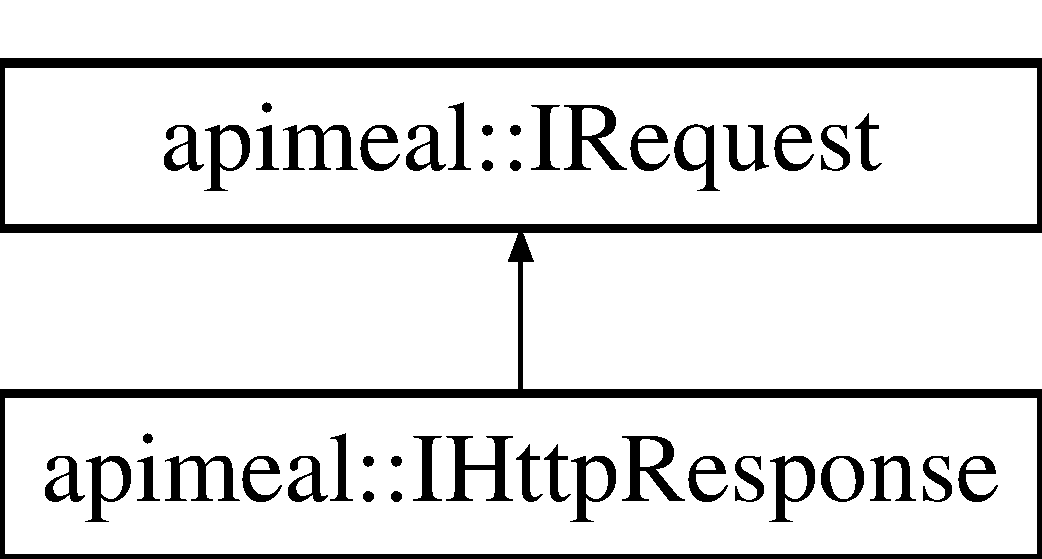
\includegraphics[height=2.000000cm]{classapimeal_1_1IHttpResponse}
\end{center}
\end{figure}
\subsection*{Public Member Functions}
\begin{DoxyCompactItemize}
\item 
virtual void \hyperlink{classapimeal_1_1IHttpResponse_aaf76ae8138e5c479804f54a3bd0ab78b}{set\-Status\-Code} (int)=0
\begin{DoxyCompactList}\small\item\em set\-Status\-Code \end{DoxyCompactList}\item 
virtual int \hyperlink{classapimeal_1_1IHttpResponse_a66455ecf6c9f5920bff33994eb3f0953}{get\-Status\-Code} () const =0
\begin{DoxyCompactList}\small\item\em get\-Status\-Code \end{DoxyCompactList}\item 
virtual void \hyperlink{classapimeal_1_1IHttpResponse_a4dd9ad19f35488e9f1542d2718b122bd}{set\-Reason\-Phrase} (std\-::string const \&)=0
\begin{DoxyCompactList}\small\item\em set\-Reason\-Phrase \end{DoxyCompactList}\item 
virtual std\-::string const \& \hyperlink{classapimeal_1_1IHttpResponse_a305d866a495d4ca04a5ccefb245457b2}{get\-Reason\-Phrase} () const =0
\begin{DoxyCompactList}\small\item\em get\-Reason\-Phrase \end{DoxyCompactList}\end{DoxyCompactItemize}


\subsection{Detailed Description}
class for create an response request 

\subsection{Member Function Documentation}
\hypertarget{classapimeal_1_1IHttpResponse_a305d866a495d4ca04a5ccefb245457b2}{\index{apimeal\-::\-I\-Http\-Response@{apimeal\-::\-I\-Http\-Response}!get\-Reason\-Phrase@{get\-Reason\-Phrase}}
\index{get\-Reason\-Phrase@{get\-Reason\-Phrase}!apimeal::IHttpResponse@{apimeal\-::\-I\-Http\-Response}}
\subsubsection[{get\-Reason\-Phrase}]{\setlength{\rightskip}{0pt plus 5cm}virtual std\-::string const\& apimeal\-::\-I\-Http\-Response\-::get\-Reason\-Phrase (
\begin{DoxyParamCaption}
{}
\end{DoxyParamCaption}
) const\hspace{0.3cm}{\ttfamily [pure virtual]}}}\label{classapimeal_1_1IHttpResponse_a305d866a495d4ca04a5ccefb245457b2}


get\-Reason\-Phrase 

\begin{DoxyReturn}{Returns}
std\-::string const \& \-: the reason phrase 
\end{DoxyReturn}
\hypertarget{classapimeal_1_1IHttpResponse_a66455ecf6c9f5920bff33994eb3f0953}{\index{apimeal\-::\-I\-Http\-Response@{apimeal\-::\-I\-Http\-Response}!get\-Status\-Code@{get\-Status\-Code}}
\index{get\-Status\-Code@{get\-Status\-Code}!apimeal::IHttpResponse@{apimeal\-::\-I\-Http\-Response}}
\subsubsection[{get\-Status\-Code}]{\setlength{\rightskip}{0pt plus 5cm}virtual int apimeal\-::\-I\-Http\-Response\-::get\-Status\-Code (
\begin{DoxyParamCaption}
{}
\end{DoxyParamCaption}
) const\hspace{0.3cm}{\ttfamily [pure virtual]}}}\label{classapimeal_1_1IHttpResponse_a66455ecf6c9f5920bff33994eb3f0953}


get\-Status\-Code 

\begin{DoxyReturn}{Returns}
int \-: return code 
\end{DoxyReturn}
\hypertarget{classapimeal_1_1IHttpResponse_a4dd9ad19f35488e9f1542d2718b122bd}{\index{apimeal\-::\-I\-Http\-Response@{apimeal\-::\-I\-Http\-Response}!set\-Reason\-Phrase@{set\-Reason\-Phrase}}
\index{set\-Reason\-Phrase@{set\-Reason\-Phrase}!apimeal::IHttpResponse@{apimeal\-::\-I\-Http\-Response}}
\subsubsection[{set\-Reason\-Phrase}]{\setlength{\rightskip}{0pt plus 5cm}virtual void apimeal\-::\-I\-Http\-Response\-::set\-Reason\-Phrase (
\begin{DoxyParamCaption}
\item[{std\-::string const \&}]{}
\end{DoxyParamCaption}
)\hspace{0.3cm}{\ttfamily [pure virtual]}}}\label{classapimeal_1_1IHttpResponse_a4dd9ad19f35488e9f1542d2718b122bd}


set\-Reason\-Phrase 


\begin{DoxyParams}{Parameters}
{\em std\-::string} & const \& \-: the reason phrase \\
\hline
\end{DoxyParams}
\hypertarget{classapimeal_1_1IHttpResponse_aaf76ae8138e5c479804f54a3bd0ab78b}{\index{apimeal\-::\-I\-Http\-Response@{apimeal\-::\-I\-Http\-Response}!set\-Status\-Code@{set\-Status\-Code}}
\index{set\-Status\-Code@{set\-Status\-Code}!apimeal::IHttpResponse@{apimeal\-::\-I\-Http\-Response}}
\subsubsection[{set\-Status\-Code}]{\setlength{\rightskip}{0pt plus 5cm}virtual void apimeal\-::\-I\-Http\-Response\-::set\-Status\-Code (
\begin{DoxyParamCaption}
\item[{int}]{}
\end{DoxyParamCaption}
)\hspace{0.3cm}{\ttfamily [pure virtual]}}}\label{classapimeal_1_1IHttpResponse_aaf76ae8138e5c479804f54a3bd0ab78b}


set\-Status\-Code 


\begin{DoxyParams}{Parameters}
{\em int} & code \-: return code \\
\hline
\end{DoxyParams}


The documentation for this class was generated from the following file\-:\begin{DoxyCompactItemize}
\item 
/home/corpille/\-Documents/\-Zia/apimeal/include/apimeal/I\-Http\-Response.\-hpp\end{DoxyCompactItemize}

\hypertarget{classapimeal_1_1ILogger}{\section{apimeal\-:\-:I\-Logger Class Reference}
\label{classapimeal_1_1ILogger}\index{apimeal\-::\-I\-Logger@{apimeal\-::\-I\-Logger}}
}


class for logger  




{\ttfamily \#include $<$I\-Logger.\-hpp$>$}

\subsection*{Public Member Functions}
\begin{DoxyCompactItemize}
\item 
\hypertarget{classapimeal_1_1ILogger_acc7484a23738886326805dfca3988c68}{virtual \hyperlink{classapimeal_1_1ILogger_acc7484a23738886326805dfca3988c68}{$\sim$\-I\-Logger} ()}\label{classapimeal_1_1ILogger_acc7484a23738886326805dfca3988c68}

\begin{DoxyCompactList}\small\item\em Destructor. \end{DoxyCompactList}\item 
virtual void \hyperlink{classapimeal_1_1ILogger_a97fc60c8ddb4742f87b1748de911af84}{Log\-Error} (std\-::string const \&)=0
\begin{DoxyCompactList}\small\item\em Log\-Error \-: method to write in the \hyperlink{structapimeal_1_1Error}{Error} mode. \end{DoxyCompactList}\item 
virtual void \hyperlink{classapimeal_1_1ILogger_a414b28b54478aab3b1cbb790d92a6dec}{Log\-Debug} (std\-::string const \&)=0
\begin{DoxyCompactList}\small\item\em Log\-Debug \-: method to write in the Debug mode. \end{DoxyCompactList}\item 
virtual void \hyperlink{classapimeal_1_1ILogger_aede6672e65066b288d112ca52a99884b}{Log\-Info} (std\-::string const \&)=0
\begin{DoxyCompactList}\small\item\em Log\-Info \-: method to write in the Info mode. \end{DoxyCompactList}\end{DoxyCompactItemize}


\subsection{Detailed Description}
class for logger 

\subsection{Member Function Documentation}
\hypertarget{classapimeal_1_1ILogger_a414b28b54478aab3b1cbb790d92a6dec}{\index{apimeal\-::\-I\-Logger@{apimeal\-::\-I\-Logger}!Log\-Debug@{Log\-Debug}}
\index{Log\-Debug@{Log\-Debug}!apimeal::ILogger@{apimeal\-::\-I\-Logger}}
\subsubsection[{Log\-Debug}]{\setlength{\rightskip}{0pt plus 5cm}virtual void apimeal\-::\-I\-Logger\-::\-Log\-Debug (
\begin{DoxyParamCaption}
\item[{std\-::string const \&}]{}
\end{DoxyParamCaption}
)\hspace{0.3cm}{\ttfamily [pure virtual]}}}\label{classapimeal_1_1ILogger_a414b28b54478aab3b1cbb790d92a6dec}


Log\-Debug \-: method to write in the Debug mode. 


\begin{DoxyParams}{Parameters}
{\em std\-::string} & const \& \\
\hline
\end{DoxyParams}
\hypertarget{classapimeal_1_1ILogger_a97fc60c8ddb4742f87b1748de911af84}{\index{apimeal\-::\-I\-Logger@{apimeal\-::\-I\-Logger}!Log\-Error@{Log\-Error}}
\index{Log\-Error@{Log\-Error}!apimeal::ILogger@{apimeal\-::\-I\-Logger}}
\subsubsection[{Log\-Error}]{\setlength{\rightskip}{0pt plus 5cm}virtual void apimeal\-::\-I\-Logger\-::\-Log\-Error (
\begin{DoxyParamCaption}
\item[{std\-::string const \&}]{}
\end{DoxyParamCaption}
)\hspace{0.3cm}{\ttfamily [pure virtual]}}}\label{classapimeal_1_1ILogger_a97fc60c8ddb4742f87b1748de911af84}


Log\-Error \-: method to write in the \hyperlink{structapimeal_1_1Error}{Error} mode. 


\begin{DoxyParams}{Parameters}
{\em std\-::string} & const \& \\
\hline
\end{DoxyParams}
\hypertarget{classapimeal_1_1ILogger_aede6672e65066b288d112ca52a99884b}{\index{apimeal\-::\-I\-Logger@{apimeal\-::\-I\-Logger}!Log\-Info@{Log\-Info}}
\index{Log\-Info@{Log\-Info}!apimeal::ILogger@{apimeal\-::\-I\-Logger}}
\subsubsection[{Log\-Info}]{\setlength{\rightskip}{0pt plus 5cm}virtual void apimeal\-::\-I\-Logger\-::\-Log\-Info (
\begin{DoxyParamCaption}
\item[{std\-::string const \&}]{}
\end{DoxyParamCaption}
)\hspace{0.3cm}{\ttfamily [pure virtual]}}}\label{classapimeal_1_1ILogger_aede6672e65066b288d112ca52a99884b}


Log\-Info \-: method to write in the Info mode. 


\begin{DoxyParams}{Parameters}
{\em std\-::string} & const \& \\
\hline
\end{DoxyParams}


The documentation for this class was generated from the following file\-:\begin{DoxyCompactItemize}
\item 
/home/corpille/\-Documents/\-Zia/apimeal/include/apimeal/I\-Logger.\-hpp\end{DoxyCompactItemize}

\hypertarget{classapimeal_1_1IRequest}{\section{apimeal\-:\-:I\-Request Class Reference}
\label{classapimeal_1_1IRequest}\index{apimeal\-::\-I\-Request@{apimeal\-::\-I\-Request}}
}


content of a query  




{\ttfamily \#include $<$I\-Request.\-hpp$>$}

Inheritance diagram for apimeal\-:\-:I\-Request\-:\begin{figure}[H]
\begin{center}
\leavevmode
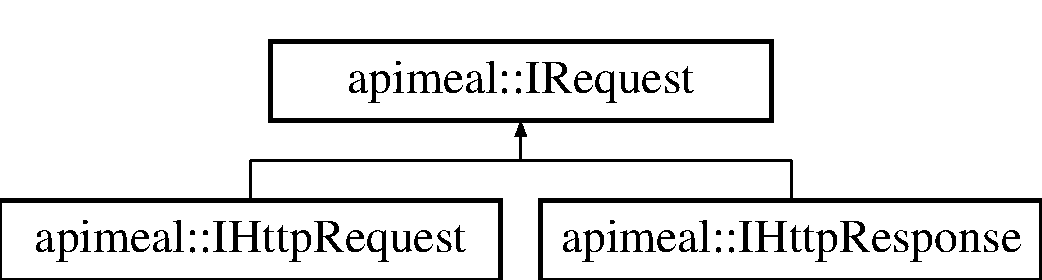
\includegraphics[height=2.000000cm]{classapimeal_1_1IRequest}
\end{center}
\end{figure}
\subsection*{Public Member Functions}
\begin{DoxyCompactItemize}
\item 
\hypertarget{classapimeal_1_1IRequest_a200a902019f7ef0272866d29a00feed6}{virtual \hyperlink{classapimeal_1_1IRequest_a200a902019f7ef0272866d29a00feed6}{$\sim$\-I\-Request} ()}\label{classapimeal_1_1IRequest_a200a902019f7ef0272866d29a00feed6}

\begin{DoxyCompactList}\small\item\em Destructor. \end{DoxyCompactList}\item 
virtual void \hyperlink{classapimeal_1_1IRequest_a91098a447ab3b6cc035dd4fd789e5ae6}{set\-Body} (std\-::string const \&)=0
\begin{DoxyCompactList}\small\item\em set\-Body \-: set the body \end{DoxyCompactList}\item 
virtual std\-::string const \& \hyperlink{classapimeal_1_1IRequest_ae960126642019a346b99b25401d8227a}{get\-Body} () const =0
\begin{DoxyCompactList}\small\item\em get\-Body \-: get the body \end{DoxyCompactList}\item 
virtual std\-::map$<$ std\-::string, \\*
std\-::string $>$ const \& \hyperlink{classapimeal_1_1IRequest_ae1570e7bce31e01b19a44d2b1552ee1a}{get\-Headers} () const =0
\begin{DoxyCompactList}\small\item\em get\-Headers \-: get the headers \end{DoxyCompactList}\item 
virtual void \hyperlink{classapimeal_1_1IRequest_a6561e8a6ec011ac8e23ec2e9a2007ee5}{add\-Header} (std\-::string const \&key, std\-::string const \&value)=0
\begin{DoxyCompactList}\small\item\em add\-Headers \-: adding a line in the header \end{DoxyCompactList}\item 
virtual void \hyperlink{classapimeal_1_1IRequest_a6721f40bf978b65fe16c391be6de5ee6}{set\-Headers} (std\-::map$<$ std\-::string, std\-::string $>$ const \&headers)=0
\begin{DoxyCompactList}\small\item\em set\-Headers \-: set the header \end{DoxyCompactList}\item 
virtual void \hyperlink{classapimeal_1_1IRequest_aa2e8c5d8e3ea03dfd9d4a85fa36ad25b}{remove\-Header} (std\-::string const \&key)=0
\begin{DoxyCompactList}\small\item\em remove\-Header \-: removing a line in the header \end{DoxyCompactList}\end{DoxyCompactItemize}


\subsection{Detailed Description}
content of a query 

\subsection{Member Function Documentation}
\hypertarget{classapimeal_1_1IRequest_a6561e8a6ec011ac8e23ec2e9a2007ee5}{\index{apimeal\-::\-I\-Request@{apimeal\-::\-I\-Request}!add\-Header@{add\-Header}}
\index{add\-Header@{add\-Header}!apimeal::IRequest@{apimeal\-::\-I\-Request}}
\subsubsection[{add\-Header}]{\setlength{\rightskip}{0pt plus 5cm}virtual void apimeal\-::\-I\-Request\-::add\-Header (
\begin{DoxyParamCaption}
\item[{std\-::string const \&}]{key, }
\item[{std\-::string const \&}]{value}
\end{DoxyParamCaption}
)\hspace{0.3cm}{\ttfamily [pure virtual]}}}\label{classapimeal_1_1IRequest_a6561e8a6ec011ac8e23ec2e9a2007ee5}


add\-Headers \-: adding a line in the header 


\begin{DoxyParams}{Parameters}
{\em std\-::string} & const\& key \\
\hline
{\em std\-::string} & const\& value \\
\hline
\end{DoxyParams}
\hypertarget{classapimeal_1_1IRequest_ae960126642019a346b99b25401d8227a}{\index{apimeal\-::\-I\-Request@{apimeal\-::\-I\-Request}!get\-Body@{get\-Body}}
\index{get\-Body@{get\-Body}!apimeal::IRequest@{apimeal\-::\-I\-Request}}
\subsubsection[{get\-Body}]{\setlength{\rightskip}{0pt plus 5cm}virtual std\-::string const\& apimeal\-::\-I\-Request\-::get\-Body (
\begin{DoxyParamCaption}
{}
\end{DoxyParamCaption}
) const\hspace{0.3cm}{\ttfamily [pure virtual]}}}\label{classapimeal_1_1IRequest_ae960126642019a346b99b25401d8227a}


get\-Body \-: get the body 

\begin{DoxyReturn}{Returns}
std\-::string const \& body 
\end{DoxyReturn}
\hypertarget{classapimeal_1_1IRequest_ae1570e7bce31e01b19a44d2b1552ee1a}{\index{apimeal\-::\-I\-Request@{apimeal\-::\-I\-Request}!get\-Headers@{get\-Headers}}
\index{get\-Headers@{get\-Headers}!apimeal::IRequest@{apimeal\-::\-I\-Request}}
\subsubsection[{get\-Headers}]{\setlength{\rightskip}{0pt plus 5cm}virtual std\-::map$<$std\-::string, std\-::string$>$ const\& apimeal\-::\-I\-Request\-::get\-Headers (
\begin{DoxyParamCaption}
{}
\end{DoxyParamCaption}
) const\hspace{0.3cm}{\ttfamily [pure virtual]}}}\label{classapimeal_1_1IRequest_ae1570e7bce31e01b19a44d2b1552ee1a}


get\-Headers \-: get the headers 

\begin{DoxyReturn}{Returns}
std\-::map$<$std\-::string, std\-::string$>$ const \& header \-: example (key \-: \char`\"{}\-User-\/\-Agent\char`\"{} val \-: \char`\"{}curl\char`\"{}) 
\end{DoxyReturn}
\hypertarget{classapimeal_1_1IRequest_aa2e8c5d8e3ea03dfd9d4a85fa36ad25b}{\index{apimeal\-::\-I\-Request@{apimeal\-::\-I\-Request}!remove\-Header@{remove\-Header}}
\index{remove\-Header@{remove\-Header}!apimeal::IRequest@{apimeal\-::\-I\-Request}}
\subsubsection[{remove\-Header}]{\setlength{\rightskip}{0pt plus 5cm}virtual void apimeal\-::\-I\-Request\-::remove\-Header (
\begin{DoxyParamCaption}
\item[{std\-::string const \&}]{key}
\end{DoxyParamCaption}
)\hspace{0.3cm}{\ttfamily [pure virtual]}}}\label{classapimeal_1_1IRequest_aa2e8c5d8e3ea03dfd9d4a85fa36ad25b}


remove\-Header \-: removing a line in the header 


\begin{DoxyParams}{Parameters}
{\em std\-::string} & const \&key \\
\hline
\end{DoxyParams}
\hypertarget{classapimeal_1_1IRequest_a91098a447ab3b6cc035dd4fd789e5ae6}{\index{apimeal\-::\-I\-Request@{apimeal\-::\-I\-Request}!set\-Body@{set\-Body}}
\index{set\-Body@{set\-Body}!apimeal::IRequest@{apimeal\-::\-I\-Request}}
\subsubsection[{set\-Body}]{\setlength{\rightskip}{0pt plus 5cm}virtual void apimeal\-::\-I\-Request\-::set\-Body (
\begin{DoxyParamCaption}
\item[{std\-::string const \&}]{}
\end{DoxyParamCaption}
)\hspace{0.3cm}{\ttfamily [pure virtual]}}}\label{classapimeal_1_1IRequest_a91098a447ab3b6cc035dd4fd789e5ae6}


set\-Body \-: set the body 


\begin{DoxyParams}{Parameters}
{\em std\-::string} & const \& body \\
\hline
\end{DoxyParams}
\hypertarget{classapimeal_1_1IRequest_a6721f40bf978b65fe16c391be6de5ee6}{\index{apimeal\-::\-I\-Request@{apimeal\-::\-I\-Request}!set\-Headers@{set\-Headers}}
\index{set\-Headers@{set\-Headers}!apimeal::IRequest@{apimeal\-::\-I\-Request}}
\subsubsection[{set\-Headers}]{\setlength{\rightskip}{0pt plus 5cm}virtual void apimeal\-::\-I\-Request\-::set\-Headers (
\begin{DoxyParamCaption}
\item[{std\-::map$<$ std\-::string, std\-::string $>$ const \&}]{headers}
\end{DoxyParamCaption}
)\hspace{0.3cm}{\ttfamily [pure virtual]}}}\label{classapimeal_1_1IRequest_a6721f40bf978b65fe16c391be6de5ee6}


set\-Headers \-: set the header 


\begin{DoxyParams}{Parameters}
{\em std\-::map$<$std\-::string,std\-::string$>$} & const \& header \-: example (key \-: \char`\"{}\-User-\/\-Agent\char`\"{} val \-: \char`\"{}curl\char`\"{}) \\
\hline
\end{DoxyParams}


The documentation for this class was generated from the following file\-:\begin{DoxyCompactItemize}
\item 
/home/corpille/\-Documents/\-Zia/apimeal/include/apimeal/I\-Request.\-hpp\end{DoxyCompactItemize}

\hypertarget{structapimeal_1_1Version}{\section{apimeal\-:\-:Version Struct Reference}
\label{structapimeal_1_1Version}\index{apimeal\-::\-Version@{apimeal\-::\-Version}}
}


Set the slice versions compatible with the module.  




{\ttfamily \#include $<$Version.\-hpp$>$}

\subsection*{Public Member Functions}
\begin{DoxyCompactItemize}
\item 
\hypertarget{structapimeal_1_1Version_a2709f76d935fe5d194b469a9923b515d}{{\bfseries Version} (int ma, int mi)}\label{structapimeal_1_1Version_a2709f76d935fe5d194b469a9923b515d}

\end{DoxyCompactItemize}
\subsection*{Public Attributes}
\begin{DoxyCompactItemize}
\item 
\hypertarget{structapimeal_1_1Version_a12307d3b608a391a289fd5c3d4e74be2}{int {\bfseries Major}}\label{structapimeal_1_1Version_a12307d3b608a391a289fd5c3d4e74be2}

\item 
\hypertarget{structapimeal_1_1Version_a9f2c4435c4b0d848a7a6731f30dc4aaf}{int {\bfseries Minor}}\label{structapimeal_1_1Version_a9f2c4435c4b0d848a7a6731f30dc4aaf}

\end{DoxyCompactItemize}


\subsection{Detailed Description}
Set the slice versions compatible with the module. 


\begin{DoxyParams}{Parameters}
{\em int} & max \\
\hline
{\em int} & min \\
\hline
\end{DoxyParams}


The documentation for this struct was generated from the following file\-:\begin{DoxyCompactItemize}
\item 
/home/corpille/\-Documents/\-Zia/apimeal/include/apimeal/Version.\-hpp\end{DoxyCompactItemize}

%--- End generated contents ---

% Index
\newpage
\phantomsection
\addcontentsline{toc}{part}{Index}
\printindex

\end{document}
